% !TEX program = pdflatex
% IEEE Transactions on Power Systems -- modular energy-structured reduced model
% Compile: pdflatex -> bibtex -> pdflatex -> pdflatex.
%   Bibliography in bib/references.bib.
%
% v1.1 (2026-09-04): full rewrite on the real kiki corpus (results/e02..e08,
%   reports/synthesis_paper_main.md); earlier body (7-area aggregation, M2a,
%   M2A-LYAP) reported superseded results and MUST NOT be cited. Real figures
%   wired (figures/fig{1,2,3}_*.pdf, generated from frozen models and immutable
%   results by experiments/paper_figures.py); bibliography switched to bibtex.

\documentclass[journal]{IEEEtran}

\usepackage{cite}
\usepackage{amsmath,amssymb,amsfonts}
\usepackage{algorithmic}
\usepackage{graphicx}
\usepackage{textcomp}
\usepackage{xcolor}
\usepackage{booktabs}
\usepackage{array}
\usepackage{multirow}
\usepackage{url}
\usepackage{balance}

\newcommand{\diag}{\operatorname{diag}}
\newcommand{\softplus}{\operatorname{softplus}}
\newcommand{\R}{\mathbb{R}}
\graphicspath{{figures/}}

\hyphenation{op-tical net-works semi-conduc-tor power-sys-tems closed-loop}

\begin{document}

\title{Modular Symbolic Learning of Energy-Structured\\ Reduced Models with Integration-Free Candidate Screening\\ for Power-System Transients}

\author{First~A.~Author,~\IEEEmembership{Member,~IEEE,}
        Second~B.~Author,~\IEEEmembership{Senior Member,~IEEE,}
        and~Third~C.~Author,~\IEEEmembership{Fellow,~IEEE}%
\thanks{Manuscript received XX, 2026. This work was supported in part by XX.}
\thanks{First A. Author and Second B. Author are with the Department of Electrical and Computer Engineering, University Name, City, Country (e-mail: author1@example.edu).}
\thanks{Third C. Author is with Organization Name, City, Country.}
\thanks{Corresponding author: First A. Author.}}

\markboth{IEEE Transactions on Power Systems,~Vol.~XX, No.~X, Month~20XX}%
{Author \MakeLowercase{\textit{et al.}}: Modular Symbolic Learning of Energy-Structured Reduced Power-System Dynamics}

\maketitle

\begin{abstract}
Transient security assessment repeatedly integrates high-order power-system
models, while unconstrained data-driven surrogates can fail under closed-loop
rollout. We formulate cleared post-fault reduction as modular identification:
a non-removable swing backbone is augmented with reciprocal, energy-compatible
node and edge-memory ports proposed from integral residuals and admitted by a
source-stratified deletion gate. The fitted model has an explicit storage
function whose centering, stationarity, local curvature, and supply identity can
be audited numerically. A local search for low-energy boundary and saddle
candidates then supplies an integration-free clearing-state \emph{screen}. It
does not establish the globally verified escape-energy lower bound required for
a stability certificate. On a previously analyzed 315-event IEEE~39-bus build,
the retrospective screen did not label any of 51 unstable events as stable; the
events represent only nine source/fault-line groups, giving a one-sided 95\%
exact upper bound of 0.283 on the group miss probability, at 0.23 stable-event
coverage. These values and the inherited trajectory/baseline comparisons are
exploratory because the build was opened by multiple legacy analyses. We
therefore preregister a single-pass release that fixes all endpoints, uses final
gate-compliant models, and permanently records access before reading a genuinely
fresh holdout. That release remains blocked; no confirmatory out-of-sample claim
is made here.
\end{abstract}

\begin{IEEEkeywords}
Transient stability assessment, reduced-order modeling, sparse symbolic
identification, energy function, Lyapunov methods, model selection, oscillation
modes.
\end{IEEEkeywords}

% =====================================================================
\section{Introduction}
% =====================================================================

\IEEEPARstart{P}{ower-system} dynamic studies use high-order
differential-algebraic models that include synchronous-machine electrical
states, exciters, governors, and network constraints~\cite{kundur1994}.
Repeated integration of such models is the workhorse of transient stability
assessment, but the cost grows quickly with system size, contingency count, and
horizon. Two complementary lines of research try to cut that cost: reduced
dynamic models that summarize the electromechanical response, and direct
(energy-based) stability criteria that avoid integration altogether.

Reduced-order dynamic equivalents have a long history, from coherency-based
aggregation~\cite{chow2013coherency} and structure-preserving energy
formulations~\cite{bergen1981structure} to balanced and measurement-based
reductions. These approaches usually \emph{fix} the reduced equation class a
priori (typically a classical swing or aggregated model) rather than deciding
from data which physical effects a reduced model must retain. On a separate
axis, direct methods construct an energy or Lyapunov function for a given model
and compare the fault-cleared state against the energy of a critical
point~\cite{pai1989energy,chiang2011direct}. Their accuracy is limited in
practice by the need for an accurate model that already possesses a valid
energy function, which is precisely what data-driven surrogates do not provide.

Equation discovery offers a data-driven route to the model itself. Sparse
identification of nonlinear dynamics (SINDy)~\cite{brunton2016sindy} regresses a
candidate symbolic library against measured derivatives and keeps only the
dominant terms. Weak-form integral variants~\cite{messenger2021wsindy} and
structured sparse regressions~\cite{loiseau2018constrained} reduce the noise
amplification of differentiation, and symbolic regression has been used to
refine power-system dynamic models from data~\cite{saric2021symbolic}. Applied
directly to cleared transients, however, these methods still return unanchored
models selected on one-step fit quality: a model that fits derivatives well can
still diverge under closed-loop multi-step reintegration, and the fitted
equations carry no structural guarantee that could anchor a stability
judgment.
Physics-informed~\cite{raissi2019pinn} and recurrent~\cite{hochreiter1997lstm}
neural closures avoid the symbolic library but inherit the last two obstacles,
and they add no interpretable model for the system operator. Dynamic mode
decomposition~\cite{schmid2010dmd} identifies oscillatory modes from
measurements, yet it estimates modal content of a \emph{given} trajectory rather
than a predictive model of the cleared dynamics.

Energy-based reasoning suggests how these threads can be joined. If a reduced
model is built so that its structure \emph{is} an energy function---a
mechanical-power input port, nonnegative dissipation, and reciprocal
energy-storing memory ports---then the passivity identity
$\dot H = \text{supply}-\text{dissipation}$ holds by construction and can be
audited numerically. The cleared-state energy can also be compared with locally
found boundary energies without transient integration, although such candidates
are not a globally verified escape-energy bound. Passivity and
port-Hamiltonian modeling of power networks provide exactly such a
vocabulary~\cite{vanderschaft2017,fiaz2013porthamiltonian}. The open
question is whether a symbolic, data-driven procedure can discover which of these
energy-compatible modules a reduced model needs, rather than assuming them.

This paper proposes a modular symbolic identification procedure for cleared
post-fault transients. A physics swing backbone on the full ten-machine
center-of-inertia (COI) coordinates is never removed. Around it we maintain a
small family of energy-compatible modules whose dynamical effect is a
low-dimensional lag or resonance on the node or edge speed signals. Candidate
modules are \emph{proposed} from derivative-free integral residuals with a
source-stratified bootstrap, jointly fitted in a weak form, and then each is
tested by whole-block deletion against a 2\% non-inferiority gate on
cross-validation rollout error. Module inclusion is therefore the model-selection
decision, and a module is kept only when the data demand it. A mechanical-power
($\Delta P_m$) equation is treated as one more such module, admitted only at
horizons where it pays for itself.

The resulting models retain an explicit storage function and an auditable supply
identity. We use that structure to define an integration-free, three-state
candidate-energy screen and to obtain oscillatory modes from a linearization.
Because legacy scripts reopened the same test build and selected attractive
modal matches, we separate the resulting exploratory evidence from a blocked,
preregistered fresh-holdout protocol.

\emph{Contributions.}
\begin{itemize}
\item \textbf{Modular selection}: a data-driven procedure in which including a
      physics module is the model choice; each candidate is compared with a
      freshly refitted backbone at physical 1/5/10~s horizons and must improve
      total validation error by at least 2\% without increasing failures.
\item \textbf{Energy-structured surrogate and integration-free screening}: a
      reduced model that keeps the backbone and modules in passivity-compatible
      form, with local energy-structure audits and a three-state candidate
      screen (screened stable / screened unstable / refused). No formal stable
      verdict is issued without a verified global escape-energy lower bound.
\item \textbf{Evidence-governed evaluation}: a preregistered release fixes the
      trajectory, screening, and complete-assignment modal endpoints, enforces
      claim-before-read access, and rejects previously consumed data builds.
\item \textbf{Negative controls}: global-polynomial SINDy, a physics-informed
      residual network, and an LSTM are compared under the same causal contract
      on a development fold; these comparisons are exploratory rather than
      confirmatory.
\end{itemize}

% =====================================================================
\section{Problem Setting and Evaluation Protocol}
\label{sec:protocol}
% =====================================================================

\subsection{Cleared post-fault dynamics}
We study the transient that follows fault clearing in a multi-machine system. An
event is defined by its clearing state and its post-clear mechanical-power plan.
All trajectories are transformed to COI coordinates to remove the common
frequency drift: for each machine $i$ with effective inertia $m_i$,
\begin{equation}
\delta_i^{\mathrm c}=\delta_i-\frac{\sum_j m_j\delta_j}{\sum_j m_j},
\qquad
\omega_i^{\mathrm c}=\omega_i-\frac{\sum_j m_j\omega_j}{\sum_j m_j},
\label{eq:coi}
\end{equation}
and the same projection is applied to power balance. We model the machines at
full resolution ($n=10$), each participating in the COI swing balance over the
complete graph of $e=n(n-1)/2=45$ candidate machine pairs.

\subsection{Causal deployment contract}
A model is trained and deployed under a causal input contract. The allowed
static inputs are the clearing state $(\delta_0,\omega_0)$, the equilibrium and
clearing mechanical powers $P_m^{\mathrm{eq}}, P_m^{\mathrm{clr}}$, the effective
masses, and the network incidence. The only time-varying exogenous input is the
mechanical power $P_m(t)$. Measured quantities such as electrical power, bus
voltages, fault-line identity, and any outcome label are forbidden as inputs.
Crucially, $P_m$ observed after clearing is treated as a \emph{training-only}
teacher signal. At deployment the mechanical power is held constant at its
clearing value,
\begin{equation}
P_m(t) = P_m^{\mathrm{clr}}, \qquad t \geq 0,
\label{eq:zoh}
\end{equation}
which we call the causal zero-order-hold (ZOH) contract. A rollout advances the
model with a shared fourth-order Runge--Kutta integrator whose internal step is
bounded by 0.01~s, over a 1~s horizon ($H{=}1$\,s, 100 steps) unless stated
otherwise.

\subsection{Difficulty-conditioned reporting}
Post-clear transients span very different regimes. We therefore condition all
trajectory and safety reporting on a difficulty level that is read from the
truth trajectory only, after freezing: $\mu = \max_t |\omega^{\mathrm c}(t)|$ over
the first post-clear second. Events with $\mu \leq 0.5$\,rad\,s$^{-1}$ are
\textbf{mild}, $0.5 < \mu \leq 1.5$ are \textbf{moderate}, and $\mu > 1.5$ are
\textbf{severe} (near-critical). Reporting by difficulty rather than by a single
pooled mean is necessary because the validation folds are gentle development
sets while the test set spans the full spectrum (Section~\ref{sec:data}).

\subsection{Data and discipline}
\label{sec:data}
We use the IEEE~39-bus (New England) canonical post-clear corpus. The events
were generated by fault clearing a high-order IEEE~39-bus model built in the
symbolic-numeric simulator ANDES with synchronous-machine, excitation, and
turbine-governor dynamics~\cite{cui2021andes,athay1979practical}. The corpus
holds 315 cleared events (264 stable, 51 unstable) from ten fault lines,
partitioned into five line-disjoint folds $F_1$--$F_5$ with 206--214 training,
37--47 validation, and 61--66 test events per fold. The validation folds are
gentle (median stable
$\max|\omega^{\mathrm c}|$ of 0.37--2.24\,rad\,s$^{-1}$ across folds), whereas
the pooled test set is full-difficulty (median 2.33\,rad\,s$^{-1}$, composition
26\% mild / 15\% moderate / 59\% severe among stable events). All numerical
legacy results below were produced from frozen fold models, but separate
trajectory, screen, and sensitivity programs subsequently reopened the same
test payloads. We therefore classify all 315-event results as retrospective and
exploratory. A new build, refitted models, and the single-pass protocol in
Section~\ref{sec:release} are required for confirmatory inference.

\subsection{Confirmatory release protocol}
\label{sec:release}
Because the canonical build has been consumed by legacy analyses, it cannot serve
as a fresh confirmatory holdout. We therefore preregister a single-pass release
that requires a dataset build absent from the consumed-build register, freezes
every endpoint before any payload read, uses only final models refitted under the
corrected total module-adoption gate, and records access to each event before its
payload is opened (claim-before-read). The release fixes three
endpoints---closed-loop trajectory accuracy, the candidate-energy screen, and
the modal endpoint under one complete assignment---and forbids post-release angle
or threshold sweeps. The release remains blocked until a genuinely new build and
gate-compliant models exist; no confirmatory out-of-sample claim is made in this
paper.

% =====================================================================
\section{Modular Energy-Structured Reduced Model}
\label{sec:model}
% =====================================================================

\subsection{Swing backbone M0 (never removed)}
\label{sec:m0}
Fig.~\ref{fig:pipeline} summarizes the procedure. A physics swing backbone that
is never removed is augmented with candidate energy-compatible modules that are
proposed from integral residuals, jointly fitted in weak form, and retained only
when whole-block deletion degrades cross-validation rollout error beyond a 2\%
source-stratified non-inferiority gate. The retained model carries an auditable
energy structure and an integration-free candidate-energy margin used only for
the screening analysis in Section~\ref{sec:results}.

\begin{figure}[!t]
  \centering
  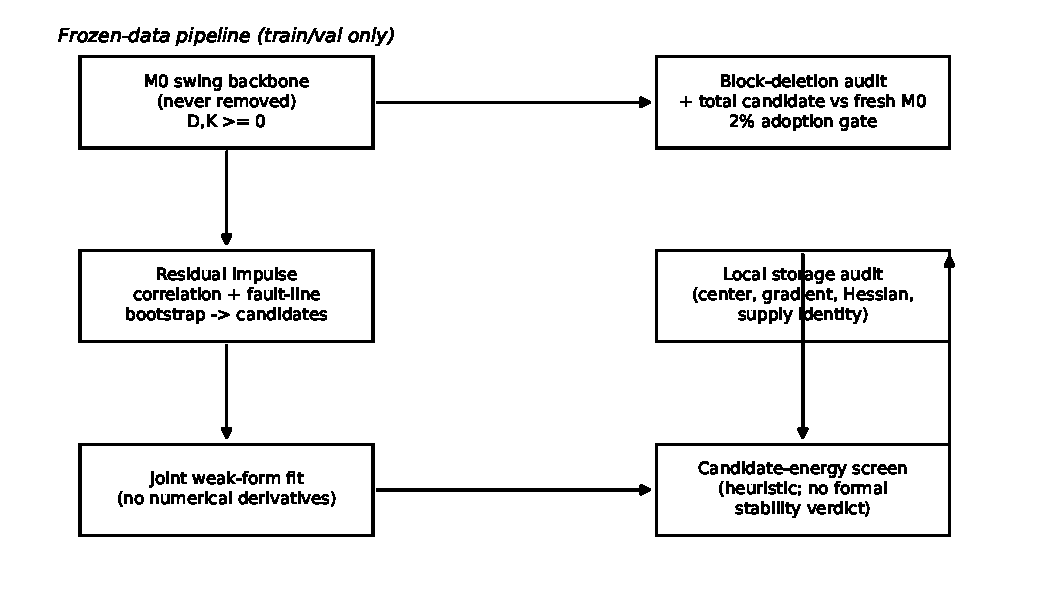
\includegraphics[width=\columnwidth]{fig1_pipeline.pdf}
  \caption{Modular identification procedure. The swing backbone is never
  removed; candidate energy-compatible modules are proposed from derivative-free
  integral residuals, fitted jointly in weak form, pruned by source-stratified
  whole-block deletion, and adopted only when the final candidate improves at
  least 2\% over a freshly refitted backbone without more failures. The
  retained model has an auditable energy structure and yields an
  integration-free candidate screen, not a stability certificate.
  Dashed arrows mark the fit-time refits after each deletion trial.}
  \label{fig:pipeline}
\end{figure}
The backbone is the classical second-order swing balance on the COI quotient,
\begin{equation}
\begin{aligned}
\dot\delta_i &= \omega_i,\\
m_i\dot\omega_i &= \Delta P_{m,i} - D_i\omega_i
- \sum_{e\in\mathcal E} B_{ie}\,
K_e\bigl(\sin\eta_e - \sin\eta_e^0\bigr),
\end{aligned}
\label{eq:backbone}
\end{equation}
where $\eta_e=\delta_i-\delta_j$ is the angle difference across machine pair
$e$, $\eta_e^0$ its pre-fault value, $B\in\R^{n\times n(n-1)/2}$ the oriented
incidence matrix of the complete candidate graph, and $\Delta
P_{m,i}=P_{m,i}-P_{m,i}^{\mathrm{eq}}$. Nonnegativity of $D_i$ and $K_e$ is
enforced by the fit. Equation~\eqref{eq:backbone} is the only component that is
never subject to deletion; everything else in the model is an optional module.

\subsection{Energy-compatible physics modules}
\label{sec:modules}
Optional modules capture physical effects that the bare backbone omits. Each
module is designed as a \emph{reciprocal passive port}: it is driven by the same
speed signal it returns force to, so its storage satisfies a port-power identity
by construction. Three module families are maintained. Define edge signals
$\nu_e=\omega_i-\omega_j=(B^{\mathsf T}\omega)_e$ and centered angles
$\theta_e=\eta_e-\eta_e^0$.

\textbf{Node high-order memory} (time constant $\tau_h{=}0.2$\,s). A per-machine
first-order state $h\in\R^n$ with nonnegative gain vector $\gamma$,
\begin{equation}
\begin{aligned}
\tau_h \dot h_i &= -h_i + \sqrt{\gamma_i}\,\omega_i,\\
f_i^{\text{node}} &= -\sqrt{\gamma_i}\,h_i,\qquad
U_h = \tfrac12\tau_h\sum_i h_i^2,
\end{aligned}
\label{eq:nodeho}
\end{equation}
adds a short electromechanical lag to the node acceleration.

\textbf{Edge memory} (time constants discovered per fold, e.g.\ 0.02/0.22/1.62~s
on $F_1$). For one instance a low-rank factor $F\in\R^{n_e\times r}$ maps edge
speed to a hidden state $z\in\R^r$,
\begin{equation}
\tau \dot z = -z + F^{\mathsf T}\nu,\qquad
f_e^{\text{edge}} = (Fz)_e,\qquad
U_m = \tfrac12\tau\, z^{\mathsf T}z,
\label{eq:edgemem}
\end{equation}
modelling a distributed, edge-wise memory of the speed difference.

\textbf{Resonant memory} (frequency/damping pairs discovered per fold, e.g.\
(0.20\,Hz, 0.49) and (0.80\,Hz, 0.10) on $F_1$). A damped oscillator with
angular frequency $\Omega=2\pi f$,
\begin{equation}
\begin{aligned}
\dot q &= p,\qquad
\dot p = F^{\mathsf T}\nu - \Omega^2 q - 2\zeta\Omega\, p,\\
f_e^{\text{osc}} &= (Fp)_e,\qquad
U_r=\tfrac12\bigl(p^{\mathsf T}p+\Omega^2 q^{\mathsf T}q\bigr),
\end{aligned}
\label{eq:resmem}
\end{equation}
adds a narrow-band oscillatory force channel. Two further families
(nonlinear edge potentials and nonlinear edge damping) are proposed by the same
procedure but received no residual support on this corpus and are not active.

Each module is attached with its port power: an edge module drawing
$\nu^{\mathsf T}(Fz)$ or $\nu^{\mathsf T}(Fp)$ from the swing appears in
\eqref{eq:backbone} as the corresponding $-B f$ term; the node module appears as
$f^{\text{node}}$. The full model is the backbone plus the active module
instances. In the inherited checkpoints these were node high-order, three
edge-memory instances, and two resonant-memory instances; those checkpoints
must be refitted under the corrected adoption gate (Section~\ref{sec:prune}).

\subsection{Module proposal from integral residuals}
\label{sec:proposal}
Candidate modules are not enumerated by hand; they are proposed from the data.
On the frozen backbone, we compute the residual impulse
\begin{equation}
\begin{aligned}
r_i ={}& \int_t^{t+W}\Delta P_{m,i}\,\mathrm d\tau
- m_i\bigl(\omega_i(t+W)-\omega_i(t)\bigr)\\
&{}-\int_t^{t+W}\Bigl(D_i\omega_i
+\sum_e B_{ie}K_e(\sin\eta_e-\sin\eta_e^0)\Bigr)\mathrm d\tau
\end{aligned}
\label{eq:resimpulse}
\end{equation}
over integration windows of widths 1--80 steps, without any numerical
differentiation. The residual is back-projected onto node and edge channels, and
each candidate mechanism is scored by the correlation of its filtered/spectral
feature with that residual, aggregated per fault-line group inside each source,
and thresholded by a source-separated bootstrap at support $\geq 0.80$. On $F_1$
this rejects nonlinear potentials and edge damping and proposes the three
time-scale memory and two resonant channels above. The median residual ratio
$|r|/\int|\Delta P_m|$ is 1.018 before modules are added. Thus the residual
impulse is comparable with the mechanical-input impulse scale; this normalized
ratio does not by itself measure a fraction of dynamics explained by the
backbone.

\subsection{Joint weak-form fitting}
\label{sec:fit}
All coefficients of the backbone and the proposed modules are estimated jointly
without numerical differentiation; this integral (weak-form) construction
follows weak-SINDy regression over integration windows~\cite{messenger2021wsindy},
but on a frozen physics backbone and with whole-block module selection. The
dynamic balance is integrated over the
same windows, producing a linear system in the coefficients whose right-hand
side is $\int\Delta P_{m}$ minus the observed momentum change $m\,\Delta\omega$.
Event weighting equalizes sources, fault lines, and events before windows. The
system is solved as a nonnegatively constrained least-squares problem in
normal-equation (Cholesky) form over a ridge grid, with an identifiability gate
(rank, equation-to-parameter ratio, condition number) and an unbiased refit of
the active support. Weak residual RMSE is $10^{-4}$--$10^{-5}$ in the per-unit
scale of the fitted equation, and physics audits (nonnegativity, COI balance,
supply identity) pass.

\subsection{Module inclusion by block pruning and total adoption}
\label{sec:prune}
Module inclusion is the model-selection step. Starting from the jointly fitted
model, instances whose reciprocal port has realized rank zero are removed
automatically. Each remaining module instance is then deleted \emph{as a whole}
and the reduced model is refitted, and the deletion is accepted only if it is
non-inferior. Concretely, for every source and horizon in
$\{1,5,10\}$\,s, the deletion must not increase rollout error beyond 2\% of the
truth variance, checked with both a point estimate and a 95\% fault-line
bootstrap upper bound over the validation fold. Any module whose deletion
degrades one source--horizon cell by more than 2\% is kept. After this internal
pruning, the \emph{entire} modular candidate is compared with a freshly refitted
backbone on the registered total validation score. It is adopted only if total
error improves by at least 2\% and its failure rate is no higher; otherwise the
whole modular candidate is rejected. The inherited $F_1$ snapshot suggests why
stratification can matter (removing the 0.80\,Hz channel degraded one long-trace
source by 39\%), but all legacy fold checkpoints predate the final total-adoption
gate and are treated as exploratory inputs to the required refit.

\subsection{$\Delta P_m$ as a gated module}
The mechanical power is a physical input, not a fitted state. Under the ZOH
contract it is constant, which is exact at very short horizons. We treat a
$\Delta P_m$ port equation as an additional candidate module: a linear
port-ODE on the zero-total-power subspace, driven by predicted relative speed,
whose spectrum is constrained to be Hurwitz with all time constants
$\leq 2.5$\,s, and whose deployment initializes from $P_m^{\mathrm{clr}}$. The
exact ZOH policy ($A{=}B{=}0$) is an explicit candidate, and the module is
admitted only when it improves total validation rollout error by $\geq$2\%
without increasing failures. Section~\ref{sec:pm} reports the legacy
horizon-dependent diagnostic.

% =====================================================================
\section{Energy-Structure Audits and the
Integration-Free Candidate Screen}
\label{sec:energy}
% =====================================================================

\subsection{Storage function}
Because the backbone potential and every module storage are of the form
(kinetic plus conservative potential plus reciprocal port storage), the model
possesses a storage function
\begin{equation}
\begin{aligned}
H(\delta,\omega,h) ={}&
\underbrace{\tfrac12\sum_i m_i\omega_i^2}_{\text{kinetic}}\\
&+
\underbrace{\sum_e K_e\bigl[\cos\eta_e^0-\cos\eta_e
-\sin\eta_e^0\,(\eta_e-\eta_e^0)\bigr]}_{\text{backbone potential}}\\
&+\sum_{\text{mod}} U_{\text{mod}}(h),
\end{aligned}
\label{eq:storage}
\end{equation}
evaluated relative to the post-clear ZOH equilibrium $\delta^{\star}$ obtained by
solving the zero-force condition of the \emph{frozen} model with
$P_m{=}P_m^{\mathrm{clr}}$; the mechanical-power tilt $\Delta
P_m^{\mathrm{clr}}$ enters as a linear potential so that $H$ vanishes at
$\delta^{\star}$. Along a ZOH rollout the passivity identity
\begin{equation}
\dot H = \underbrace{\omega^{\mathsf T}\bigl(P_m(t)-P_m^{\mathrm{clr}}\bigr)}_{\text{supply}}
-\rho(\delta,\omega,h),\qquad \rho\geq 0,
\label{eq:supply}
\end{equation}
holds with dissipation $\rho=\omega^{\mathsf T}D\omega+\omega^{\mathsf
T}B f^{\text{diss}}+\sum_{\text{mod}}\rho_{\text{mod}}$, so that under
$P_m(t)=P_m^{\mathrm{clr}}$ the storage is non-increasing along the cleared
trajectory. If the cleared storage lies strictly below a \emph{verified global
lower bound} on the energy required to escape the post-clear well, the cleared
trajectory remains bounded. Establishing such a bound is the essential
certificate step; the local optimizer used below does not establish it.

\subsection{Local energy-structure audits}
For each frozen model we audit, relative to the post-clear equilibrium, that the
storage is centered ($|H(\delta^{\star})|\approx 0$), its gradient vanishes
($\|\nabla H\|\leq 3\times10^{-10}$), the COI-projected angle/speed Hessian is
positive definite (minimum eigenvalue $\lambda_{\min}=0.1265$ in the inherited
fold artifacts), and the discrete supply identity \eqref{eq:supply} holds to
$\leq 5\times10^{-9}$. These tests audit only the named local quantities. They
do not verify hidden-state curvature, global dissipation, a region of
attraction, or a lower bound on escape energy.

\subsection{Candidate critical energy and the three-state screen}
\label{sec:margin}
For an event with clearing state $(\delta_0,\omega_0)$ under ZOH $P_m^{\mathrm
{clr}}$, the candidate critical energy is the lowest energy \emph{found} by
local search among
\begin{multline}
H_{\mathrm c}=\min\Bigl\{ H(\cdot)\ \text{at the lowest energy among}\\
\text{adjacent saddles and $\pm\eta_e=\pm\theta_{\max}$ angle boundaries}\Bigr\},
\label{eq:critical}
\end{multline}
searched over every machine pair with constrained optimization
($\theta_{\max}=\pi/2$ by default), all integration-free. The margin is
\begin{equation}
M = H_{\mathrm c} - H(\delta_0,\omega_0,h_0),
\label{eq:margin}
\end{equation}
with $h_0$ the module state consistent with $\omega_0$ at clearing. A feasible
local minimum is an upper bound on the corresponding boundary minimum, not the
global lower bound needed by the direct-method implication
\cite{chiang1987foundations,chiang1994bcu}. The margin is therefore a heuristic
screen, not a certificate. Its three reporting states are
\begin{itemize}
\item \textbf{candidate search completed and $M>0$} $\Rightarrow$ screened stable;
\item \textbf{candidate search completed and $M\leq 0$} $\Rightarrow$ screened unstable;
\item \textbf{candidate search incomplete} (no finite candidate) $\Rightarrow$
      \emph{refused} (no verdict).
\end{itemize}
The implementation always records the formal certificate status as refused
until a verified global lower bound and its assumptions are supplied.

% =====================================================================
\section{Results}
\label{sec:results}
% =====================================================================

We distinguish development, retrospective, and confirmatory evidence. Fold
validation events may be held out from coefficient fitting but participate in
hyperparameter or module selection, so they are development evidence. The
315-event build was opened by multiple legacy analyses, so its pooled trajectory
and screening values are retrospective and exploratory. No confirmatory result
exists until the preregistered release in Section~\ref{sec:release} is executed
on a fresh build. Trajectory metrics are closed-loop rollout RMSE and pooled
$R^2$; screening metrics are the fraction of truly unstable events screened
stable and the fraction of truly stable events screened stable.

\subsection{Retrospective trajectory accuracy is difficulty-conditional}
\label{sec:traj}
Table~\ref{tab:traj} reports the legacy exploratory accuracy of the frozen
modular models on 264 stable events, conditioned on difficulty. On mild
events the model reproduces the cleared transient almost exactly
(angle RMSE 0.013~rad, speed RMSE 0.069~rad\,s$^{-1}$ over the 1~s horizon);
moderate events remain accurate (0.046 and 0.190). Severe near-critical events,
whose post-clear speed excursions reach several rad\,s$^{-1}$ inside one second,
lie beyond the reduced-model domain: the error there is large and, when it
appears, conservative (the model diverges or over-declares loss of synchronism
rather than under-declaring it). The pooled mean over all stable events is
dominated by that severe majority and is not a meaningful single number.
Fig.~\ref{fig:traj} illustrates the same conditioning on development-fold
rollouts: the model tracks the mild and moderate cleared transients closely and
visibly lags only on the severe near-critical event. The numerical values have
not yet been reproduced with models refitted under the corrected total
module-adoption gate.

\begin{table}[!t]
\caption{Exploratory Accuracy of Legacy Frozen Modular Models on Stable Events
(264 of 315 events, $H{=}1$\,s ZOH rollout), by Difficulty}
\label{tab:traj}
\centering
\begin{tabular}{lccc}
\toprule
Difficulty & $n$ & Angle RMSE & Speed RMSE \\
& & (rad) & (rad\,s$^{-1}$) \\
\midrule
mild $\leq 0.5$        & 69  & 0.013 & 0.069 \\
moderate $0.5$--$1.5$  & 40  & 0.046 & 0.190 \\
severe $>1.5$          & 155 & 0.378 & 1.231 \\
\midrule
all stable             & 264 & 0.290 & 0.947 \\
\bottomrule
\end{tabular}
\par\smallskip
\parbox{\columnwidth}{\footnotesize Difficulty is the truth peak
$|\omega^{\mathrm c}|$ over the first post-clear second. A pooled speed $R^2$ is
omitted because the severe majority renders it uninformative; cross-fold speed
$R^2$ is in Table~\ref{tab:select}. RMSE is pooled over events and samples.}
\end{table}

\begin{figure}[!t]
  \centering
  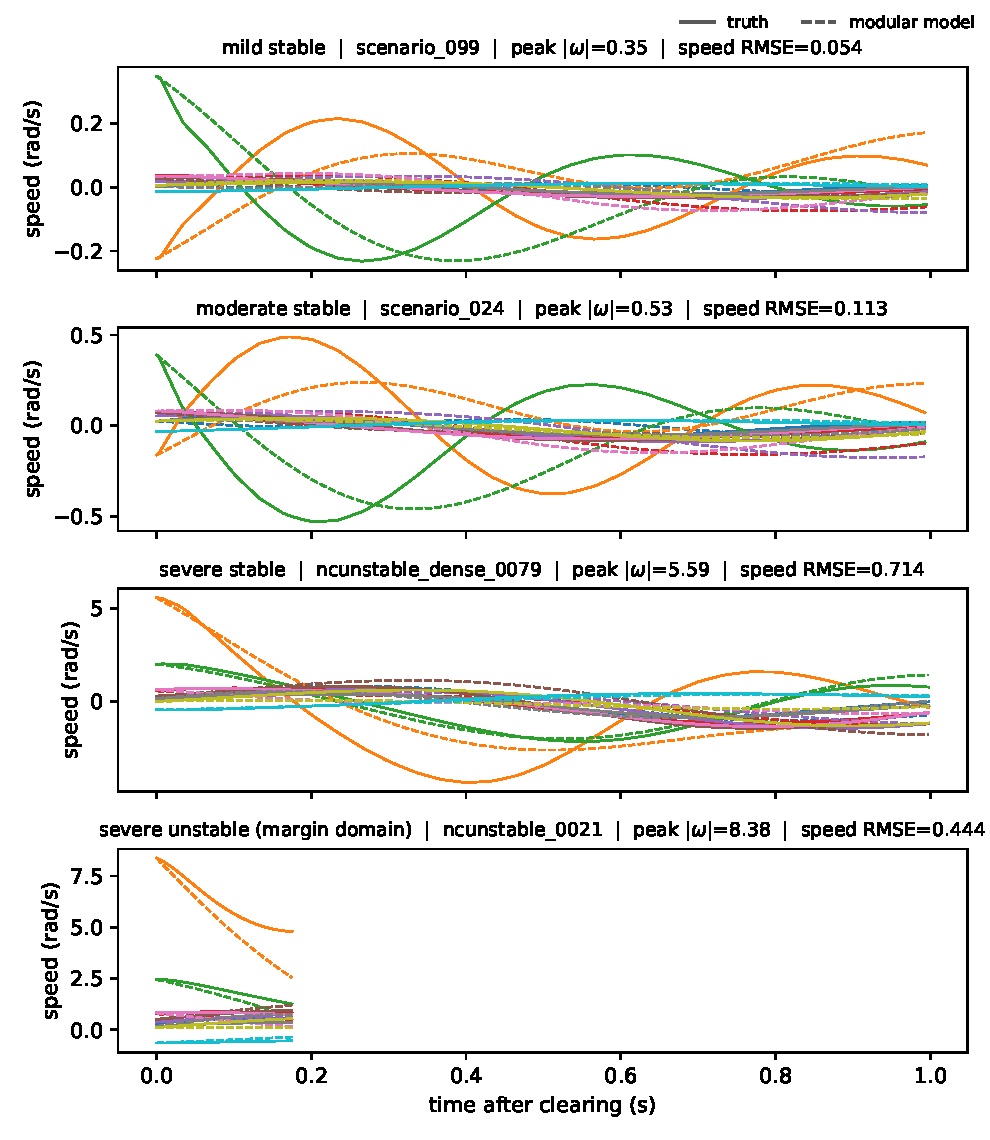
\includegraphics[width=\columnwidth]{fig2_difficulty_trajectories.pdf}
  \caption{Representative development-fold rollouts by difficulty (speed of all
  ten COI machines, truth solid vs.\ modular model dashed, $H{=}1$\,s ZOH).
  The model reproduces the mild and moderate cleared transients closely and lags
  on the severe near-critical example. The figure is a development-fold
  diagnostic; Table~\ref{tab:traj} is retrospective rather than confirmatory.}
  \label{fig:traj}
\end{figure}

\subsection{Legacy module-selection diagnostics}
\label{sec:select}
Table~\ref{tab:select} reports the inherited per-fold development snapshot that
motivated the modular construction. On the gentle and moderate development folds $F_1$--$F_3$,
addition of the proposed modules lifts the pooled speed $R^2$ of the bare
backbone from near zero or modest values to 0.70--0.80, and the whole-block
deletion audit keeps all three module families on every fold. The same modular
model is also accurate on the mild events of the severe folds. The apparent
failure on $F_4$--$F_5$ is a difficulty-composition effect, not a pipeline
inconsistency: those folds' validation sets are dominated by near-critical
events (median stable peak speeds of 1.32 and 2.24\,rad\,s$^{-1}$), which lie
outside the reduced-model domain. These checkpoints predate the corrected
comparison with a freshly refitted backbone and the total-error adoption gate;
indeed, the audited legacy $F_4$ candidate would fail the corrected total gate.
The table therefore cannot establish cross-fold selection stability and must be
recomputed before a confirmatory model claim.

\begin{table}[!t]
\caption{Legacy Cross-Fold Development Snapshot (validation, $H{=}1$\,s ZOH;
not accepted under the corrected total module-adoption gate)}
\label{tab:select}
\centering
\footnotesize
\setlength{\tabcolsep}{4pt}
\begin{tabular}{lcccccc}
\toprule
Fold & Val. & Val. stable median & Backbone & Modular & $\delta\,R^2$ & Families \\
     & $n$  & $\max|\omega^{\mathrm c}|$ & $\omega R^2$ & $\omega R^2$ & (mod.) & retained \\
\midrule
$F_1$ & 43 & 0.50 & $-0.02$ & 0.702 & 0.944 & all 3 \\
$F_2$ & 37 & 0.37 & 0.595 & 0.748 & 0.961 & all 3 \\
$F_3$ & 42 & 0.88 & 0.442 & 0.802 & 0.947 & all 3 \\
$F_4$ & 43 & 1.32 & 0.459 & $-0.031$ & 0.861 & all 3 \\
$F_5$ & 47 & 2.24 & $-3.99$ & $-2.77$ & $-0.71$ & all 3 \\
\bottomrule
\end{tabular}
\vspace{0.2em}
\footnotesize Modular column is the pruned model. Median peak speed is over
validation-stable events only (rad\,s$^{-1}$). Families: node high-order, edge
memory, resonant memory.
\end{table}

\subsection{Non-energy baselines under the same contract}
\label{sec:baselines}
We compare the modular model against three non-energy learners under the
identical causal contract on the $F_1$ development fold: (i) a global
polynomial SINDy variant (a quadratic library in angle/speed deviations and
$P_m$, fitted by one-shot least squares on time derivatives, deployed
autonomously); (ii) a physics-informed residual network whose MLP closure is
anchored at the origin and trained pointwise to the swing residual; and (iii)
    an autoregressive LSTM trained by teacher forcing. None has an explicit
    energy structure. Table~\ref{tab:baselines} reports exploratory closed-loop accuracy on the
in-domain stable events (mild and moderate). The modular model is 1.6$\times$
more accurate than its own backbone and 2.7--7.7$\times$ more accurate than the
learners that have no energy structure; the global-polynomial SINDy variant
diverges on 36 of 43 events within the 1~s horizon (non-finite rollouts). These
observations motivate, but do not prove, a structural explanation.

The key mechanism contrast is the physics-informed network. It achieves the best
\emph{pointwise} derivative fit of any learner (validation residual 0.122) yet
its closed loop is worse than the pure backbone it sits on (0.124 vs.\ 0.071
mild-plus-moderate RMSE). Pointwise fit quality therefore does not transfer to
closed-loop extrapolation. The comparison motivates structural constraints but,
because it is a bounded-budget single-fold development study, does not isolate a
unique causal mechanism.

\begin{table*}[!t]
\caption{Closed-Loop Comparison Under the Causal ZOH Contract ($F_1$ development
fold, 43 validation events, $H{=}1$\,s)}
\label{tab:baselines}
\centering
\footnotesize
\setlength{\tabcolsep}{4pt}
\begin{tabular}{lcccc}
\toprule
Model & In-domain RMSE & Severe stable & Pooled closed-loop & Energy \\
      & (mild+mod., $n{=}20$) & ($n{=}14$) & $R^2$ (all 43) & structure \\
\midrule
M0 backbone            & 0.071 & 0.882 & 0.313 & energy form \\
\textbf{modular}       & \textbf{0.045} & \textbf{0.475} & \textbf{0.797} & \textbf{audited locally} \\
Polynomial SINDy       & diverged & diverged & $-1.4\times10^{4}$ & none \\
PINN residual          & 0.124 & 0.900 & 0.278 & none \\
LSTM (autoregressive)  & 0.346 & 1.404 & $-0.90$ & none \\
\bottomrule
\end{tabular}
\par\smallskip
\parbox{\textwidth}{\footnotesize In-domain RMSE combines angle and speed RMSE
($\sqrt{(\mathrm{RMSE}_\delta^2+\mathrm{RMSE}_\omega^2)/2}$); per-state values:
M0 0.018/0.099, modular 0.012/0.063, PINN 0.061/0.164, LSTM 0.215/0.440.
Severe stable and unstable bands are outside the accuracy claim. All values are
development diagnostics and predate the current refit gate.}
\end{table*}

\subsection{Retrospective candidate-energy screen}
\label{sec:safety}
Table~\ref{tab:safety} retrospectively audits the candidate-energy screen on all
315 events. No truly unstable event was screened stable: the descriptive count
is $0/51$. Those 51 events span only nine independent source/fault-line groups;
with zero missed groups, the exact one-sided 95\% Clopper--Pearson upper bound is
0.283~\cite{clopper1934}. Of the unstable events, 41 were screened unstable and
10 refused. Only 61 of 264 stable events (23\%) were screened stable. The local
structure audits pass in the inherited fold artifacts, but they do not convert
the candidate search into a certificate. These counts describe this corpus and
are neither a zero-risk statement nor a prospective safety guarantee.

Legacy analysis also swept the candidate-energy search
angle $\theta_{\max}$. Widening it from $\pi/2$ to $0.9\pi$ raises stable
coverage from 0.23 to 0.30 (79 stable events) while keeping missed instabilities
at $0/51$ and leaving the 41 unstable-call and 10 refused decisions unchanged
event by event. Because this sweep followed access to the same data, it is
exploratory and is prohibited on the future confirmatory holdout. We retain
$\pi/2$ as the preregistered operating point. The margin is not strictly
monotone in the search angle (18 of 292 completed-search events had a smaller
margin at the wider angle), further emphasizing that this is an empirical
screen. Fig.~\ref{fig:margin} shows the retrospective screen as a function of
cleared storage and candidate critical energy.

\begin{table}[!t]
\caption{Exploratory Three-State Candidate-Energy Screen (consumed 315-event
build) and Local Structure Audits}
\label{tab:safety}
\centering
\begin{tabular}{lcc}
\toprule
Quantity & $\theta_{\max}{=}\pi/2$ & $\theta_{\max}{=}0.9\pi$ \\
\midrule
Candidate search completed  & 292 & 292 \\
Stable, screened stable     & 61  & 79 \\
Stable, unstable/refused    & 203 & 185 \\
\textbf{Missed instabilities} & \textbf{0/51} & \textbf{0/51} \\
Unstable, screened unstable & 41  & 41 \\
Unstable, refused           & 10  & 10 \\
Stable coverage             & 0.231 & 0.299 \\
\midrule
\multicolumn{3}{l}{\footnotesize Local audits (all five folds): storage centered 0,} \\
\multicolumn{3}{l}{\footnotesize $\|\nabla H(\delta^\star)\|\leq3\times10^{-10}$, projected} \\
\multicolumn{3}{l}{\footnotesize Hessian $\lambda_{\min}=0.1265>0$, supply identity} \\
\multicolumn{3}{l}{\footnotesize $\leq5\times10^{-9}$; no global escape-energy bound.}
\end{tabular}
\end{table}

\begin{figure}[!t]
  \centering
  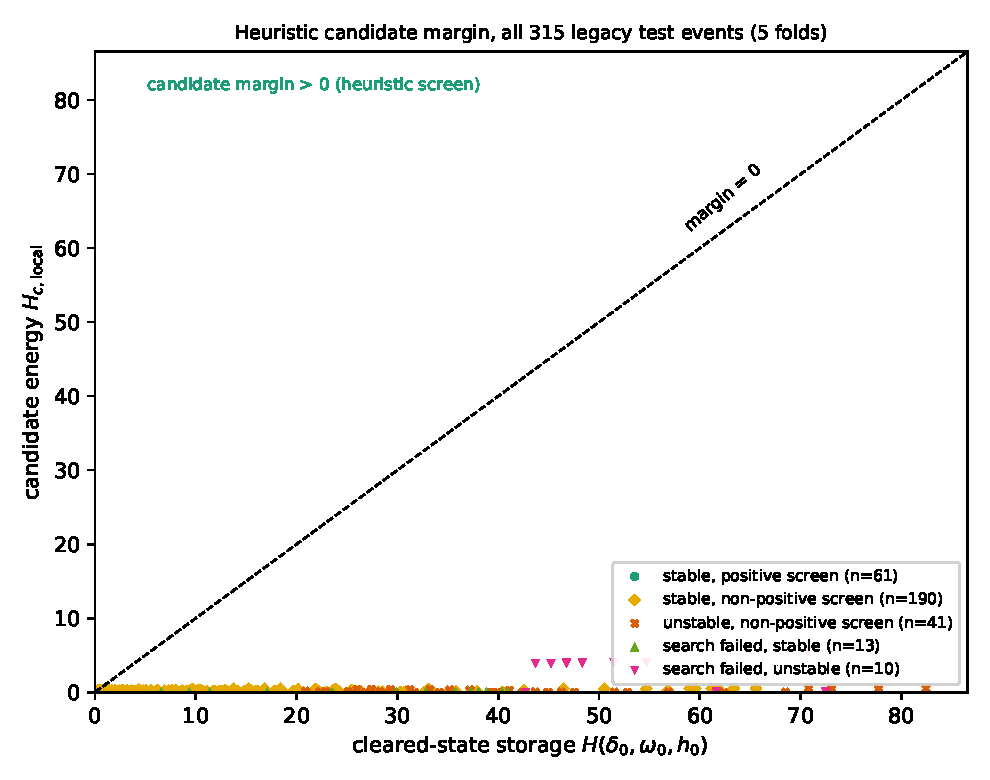
\includegraphics[width=\columnwidth]{fig3_margin_scatter.pdf}
  \caption{Exploratory integration-free screen on the consumed 315-event build:
  candidate critical energy versus cleared-state storage. The zero-margin
  diagonal separates screened-stable events (above) from screened-unstable and
  refused events (below). Screened-stable events (green) number 61. No truly
  unstable event lies in that region in this retrospective sample.}
  \label{fig:margin}
\end{figure}

\subsection{Modal endpoint under the corrected protocol}
\label{sec:modal}
The legacy modal analysis used validation-selected, pre-final models and kept
the lowest-error match within each event. Its reported frequency and damping
numbers are therefore not retained as quantitative claims. The corrected
endpoint linearizes each final pruned model at its solved post-clear equilibrium,
uses mass-weighted rotor-speed shapes, retains every pair in one complete
Hungarian assignment, computes an event median over all assigned pairs, and
macro-aggregates those event medians. This remains a post-selection validation
diagnostic until confirmed in the fresh-holdout release; current checkpoints
predate the total module-adoption gate, so no corrected modal number is reported.

\subsection{Mechanical-power module: legacy horizon-dependent diagnostic}
\label{sec:pm}
Table~\ref{tab:pm} summarizes the inherited $\Delta P_m$ development gate on the frozen backbone
at two horizons. At $H{=}1$\,s the data reject the module: even an oracle that
knows the true post-clear $P_m$ improves total RMSE by only $\sim$1\%, and the
causal ODE improves validation error by $-2.1\%$, so the exact ZOH policy is
kept. At $H{=}8$\,s the same causal gate admits the module: on the $n{=}20$ stable
events with long traces (the near-critical events, whose 8\,s transient leaves
the reduced-model domain, are excluded) raw RMSE drops from 0.0182 to 0.0118
($+35.3\%$), recovering 74\% of the gap between the ZOH policy and the
non-causal oracle. The admitted spectrum contains a slow pole with time
constant $\tau\approx2.0$\,s---consistent with the ~2.1\,s governor time
constant that physically drives the post-clear recovery---with 89 non-zero
coefficients. The snapshot suggests horizon-dependent module support, but it
predates the corrected physical-horizon and total-adoption gates and must be
rerun before being treated as an accepted model-selection result.

\begin{table}[!t]
\caption{Legacy Mechanical-Power Development Diagnostic (frozen backbone;
reported gate: $\geq$2\% validation improvement, zero failures)}
\label{tab:pm}
\centering
\begin{tabular}{lcc}
\toprule
Horizon & Verdict & Evidence \\
\midrule
$H{=}1$\,s  & \textbf{reject} ($-2.1\%$) & oracle gain only $\sim$1\%; ZOH exact \\
$H{=}8$\,s  & \textbf{adopt} ($+35.3\%$) & RMSE 0.0182$\rightarrow$0.0118; \\
           &  & recovers 74\% of ZOH$\rightarrow$oracle gap; \\
           &  & slow pole $\tau{=}2.0$\,s vs.\ governor \\
           &  & $\approx$2.1\,s; 89 non-zero coeffs. \\
\bottomrule
\end{tabular}
\vspace{0.2em}
\footnotesize The $H{=}8$\,s gate is evaluated on the $n{=}20$ stable events
with long traces; near-critical events are excluded because their long-horizon
transient leaves the reduced-model domain. This outcome-defined subset is a
reporting stratum, not a deployable selection rule.
\end{table}

% =====================================================================
\section{Discussion}
\label{sec:discussion}
% =====================================================================

The inherited development results support a structural hypothesis rather than
a confirmatory causal conclusion: reciprocal physics modules can improve
closed-loop rollout while retaining an explicit energy structure. In one
bounded-budget fold comparison, the physics-informed network had the best
pointwise derivative fit but worse closed-loop error than the backbone; the
global-polynomial SINDy variant diverged; and the LSTM drifted. This motivates
the module construction, but broader tuning and refitted cross-fold comparisons
are required before attributing the difference uniquely to structure.

\emph{What the candidate screen does and does not establish.} Because $H$ is
non-increasing along the ZOH deployment up to dissipation, cleared storage below
a \emph{verified} lower bound on the post-clear well's escape energy would imply
bounded motion. The local search supplies no such bound: a feasible candidate is
an upper bound on the corresponding boundary minimum, and the saddle search is
not proven complete. The screen is therefore empirical. Its record on the
consumed build is descriptive: no truly unstable event was screened stable
($0/51$; zero of nine independent source/fault-line groups, an exact one-sided
95\% upper bound of 0.283 on the group miss probability), and the count was
stable under the legacy $\theta_{\max}$ sweep---an exploratory finding that the
confirmatory protocol (Sec.~\ref{sec:release}) forbids repeating on a fresh
holdout. The price is coverage (0.23--0.30 of stable events), conservative by
design. A formal certificate would require a verified global escape-energy lower
bound or a BCU-type construction for this learned model; raising coverage while
keeping zero observed misses is open, and the natural fix (a bounded-trajectory
re-check of refused events) would reintroduce integration and abandon the
integration-free property.

\emph{Boundaries.} Four boundaries bound the claims. (1) The accuracy domain is
cleared post-fault transients not too close to the stability boundary; on severe
near-critical events the reduced model is not a faithful trajectory model, and
its errors there are conservative in direction. (2) The screen's stable coverage
is 0.23--0.30; screened-stable is a heuristic positive call, neither sufficient
nor necessary for a certificate, and the screen is not a complete classifier.
(3) Every accuracy number must be read by difficulty, and the pooled 315-event
mean is dominated by near-critical events and is not a headline; all such values,
and the development comparisons, are exploratory until the preregistered release
(Sec.~\ref{sec:release}) runs on a fresh build. (4) The corrected modal endpoint
is a validation diagnostic; the legacy frequency and damping values that used
per-event best matching are not retained as claims, and mode shapes do not
transfer on this data. The baselines were run with a bounded CPU budget on one
fold; more epochs would shrink the LSTM's numerical gap but would not remove its
structural limitations.

\emph{Related-work positioning.} Relative to energy-function direct methods, our
contribution is the model: we do not assume a swing-plus-uniform-damping energy,
we discover which energy-compatible modules are needed and audit the resulting
energy structure numerically. Relative to SINDy, we replace pointwise derivative
regression with weak-form integral fitting on a frozen physics backbone, and we
gate modules by closed-loop, source-stratified deletion rather than by
coefficient sparsity. Relative to physics-informed and recurrent learners, we
keep the model symbolic, interpretable, and structurally audited. The $\Delta
P_m$ experiment shows the framework also degrades gracefully: when a module is
not supported at the operating horizon, the gate keeps the clean ZOH policy and
reports the negative result rather than forcing a module in.

% =====================================================================
\section{Conclusion}
\label{sec:conclusion}
% =====================================================================

We presented a modular symbolic identification procedure for cleared post-fault
power-system dynamics in which model selection is module inclusion: a physics
swing backbone that is never removed is augmented with energy-compatible modules
proposed from integral residuals and retained only when they pass a
source-stratified, total-error adoption gate. Because the backbone
and modules are passivity-compatible, the fitted model has an auditable storage
function and supports an integration-free candidate-energy screen from the
clearing state; the local candidate search is not a verified global
escape-energy lower bound, so no formal stability certificate is issued.

On the IEEE~39-bus canonical corpus under a causal ZOH contract, inherited
development diagnostics show speed-$R^2$ gains on several gentle validation
folds, while the consumed 315-event build gives exploratory mild/moderate angle
RMSE of 0.013--0.046~rad and no unstable event screened stable ($0/51$, over nine
independent source/fault-line groups). Non-energy baselines were less accurate
in one bounded-budget development comparison. These observations are not current
confirmatory results: the stored models require refitting under the corrected
gate, and confirmatory inference awaits the preregistered single-pass release on
a fresh build.

The claims stop where the evidence stops: the accuracy domain is post-clear
transients not too close to the stability boundary; the candidate-energy screen
is a heuristic, not a certificate; and no corrected modal number is reported
until a fresh holdout exists. We intend to build a genuinely new dataset and
execute the preregistered release, to pursue a hybrid rule that re-checks refused
near-critical events with bounded trajectories, and to scale the modular
procedure to reduced coordinates for larger systems.

\balance
\bibliographystyle{IEEEtran}
\bibliography{bib/references}

\end{document}
